\documentclass[tikz,border=3mm]{standalone}
\usepackage[T1]{fontenc}
\usetikzlibrary{arrows.meta,positioning}
\begin{document}
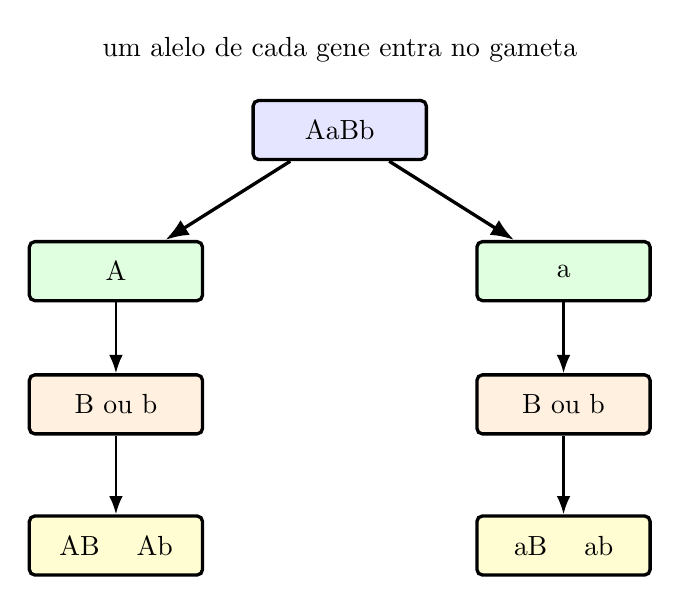
\begin{tikzpicture}[>=Latex,node distance=0.9cm]
  \tikzstyle{box}=[draw,rounded corners=2pt,very thick,minimum width=2.2cm,minimum height=0.75cm,align=center]
  \node[box,fill=blue!10] (geno) {AaBb};
  \node[box,fill=green!12,below left=1.0cm and 0.6cm of geno] (abig) {A};
  \node[box,fill=green!12,below right=1.0cm and 0.6cm of geno] (asmall) {a};
  \node[box,fill=orange!12,below=0.9cm of abig] (b1) {B ou b};
  \node[box,fill=orange!12,below=0.9cm of asmall] (b2) {B ou b};
  \node[box,fill=yellow!18,below=1.0cm of b1] (AB) {AB \quad Ab};
  \node[box,fill=yellow!18,below=1.0cm of b2] (aB) {aB \quad ab};
  \draw[very thick,->] (geno) -- (abig);
  \draw[very thick,->] (geno) -- (asmall);
  \draw[thick,->] (abig) -- (b1);
  \draw[thick,->] (asmall) -- (b2);
  \draw[thick,->] (b1) -- (AB);
  \draw[thick,->] (b2) -- (aB);
  \node[align=center,above=0.35cm of geno] {um alelo de cada gene entra no gameta};
\end{tikzpicture}
\end{document}
